\subsubsection{\newrevision{Alternative MFCC Compression and Feature-Packet Design}}
\label{sec:codec_design}
\begingroup
\color{green!45!black}
The selected architecture sends local classification results. The following codec remains a separate feature-transmission investigation and is not used by the current result-only head. The standalone \texttt{sensing/} firmware implements temporal delta, ZigZag, and coefficient-specific Rice coding for a $15\times13$ signed-int8 MFCC matrix. The codec preserves the quantized matrix and its float32 scale exactly after lossy quantization. Section~\ref{sec:codec_results} reports the host verification results.

\paragraph{Offline feature preparation}
The offline pipeline takes seconds 5--15 from recordings at least 20 s long and uses a centered 10 s clip for recordings between 10 and 20 s. Clips of 10 s or less retain their full duration. The pipeline resamples to 8 kHz and applies a zero-phase 100--2500 Hz bandpass without SNR gating or signal squaring. MFCC analysis uses 25 ms windows, 10 ms hops, a 256-point FFT, 26 Slaney Mel filters, and temporal aggregation into 15 bins with 13 coefficients each. Each recording stores 195 symmetrically quantized int8 coefficients and one float32 reconstruction scale.

\begin{figure}[htbp]
\centering
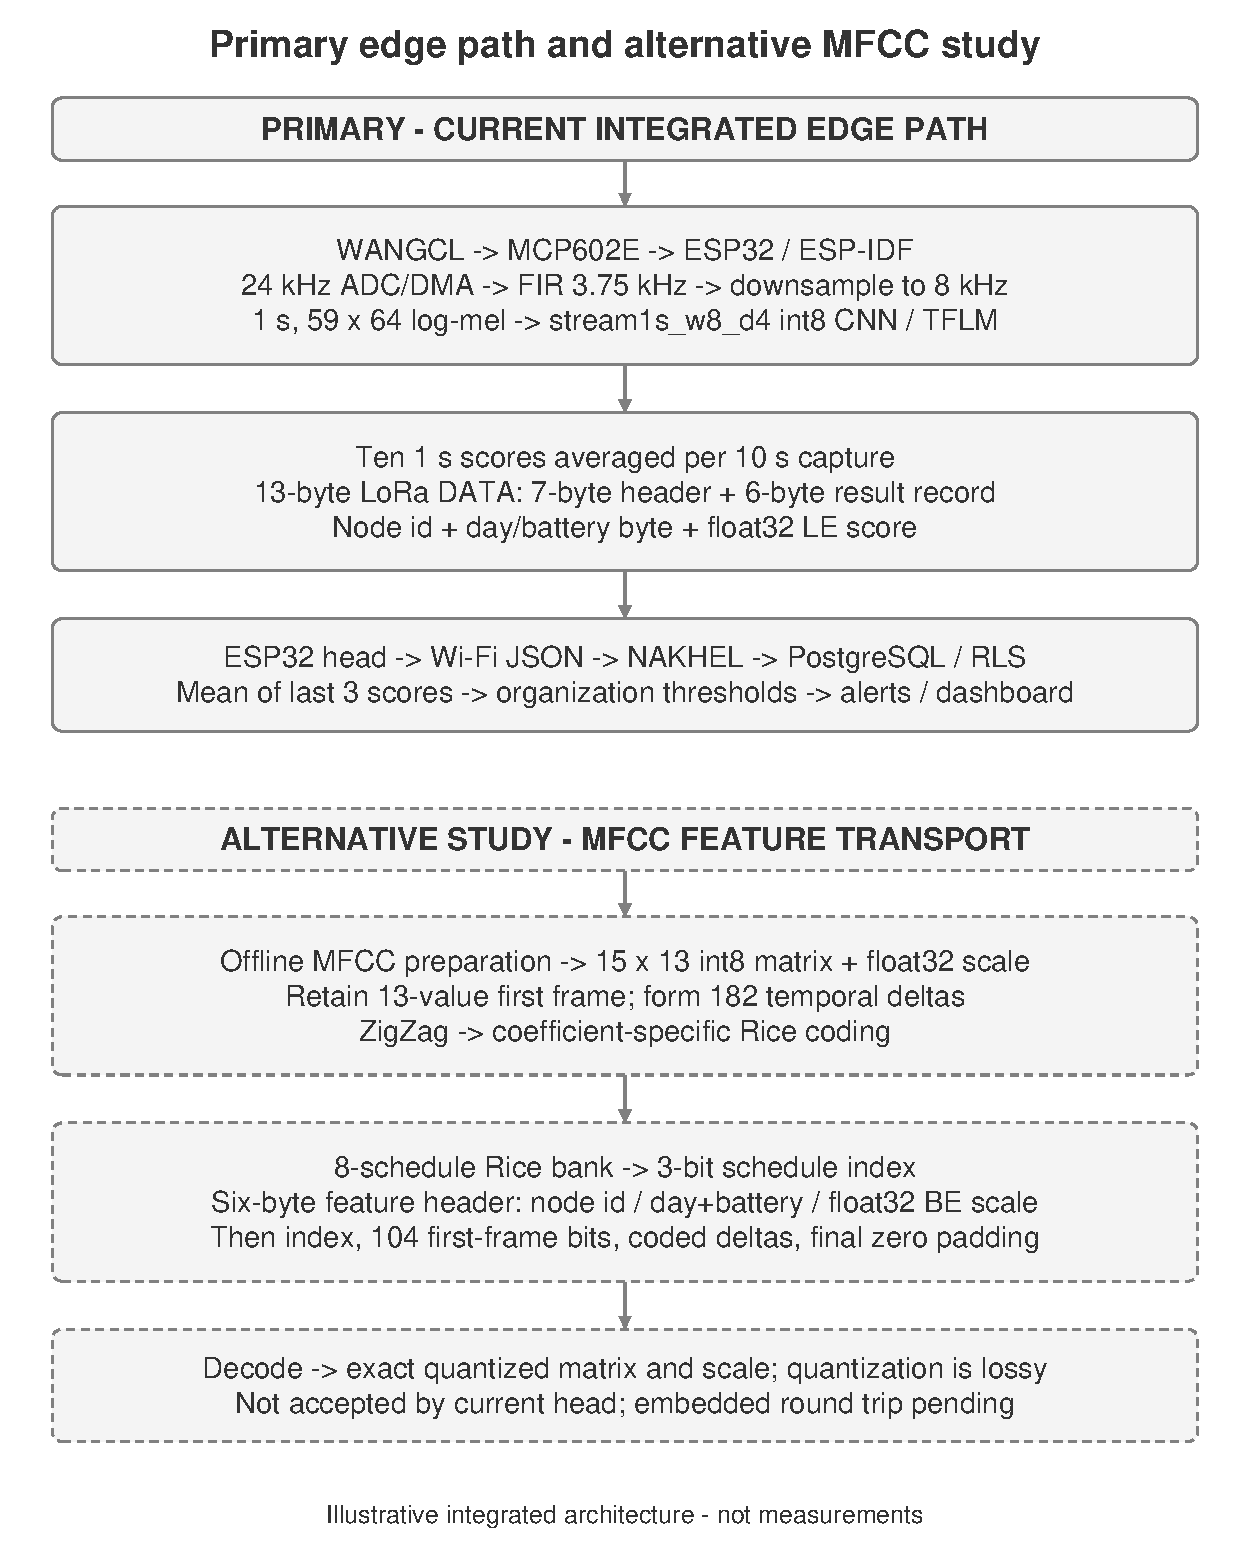
\includegraphics[width=\textwidth,height=0.78\textheight,keepaspectratio]{figures/codec_current_pipeline.pdf}
\caption{\newrevision{Selected edge-inference path alongside the alternative MFCC codec. Feature decoding is separate from the current result-forwarding protocol; exact reconstruction applies only after quantization.}}
\label{fig:codec_current_pipeline}
\end{figure}
\FloatBarrier

\paragraph{Encoding and reconstruction}
The first frame is retained as 13 raw int8 values (104 bits). For each later frame, the encoder computes
\[
d_{t,c}=\operatorname{int16}(Q_{t,c})-\operatorname{int16}(Q_{t-1,c}),\qquad
 t=1,\ldots,14,\quad c=0,\ldots,12.
\]
The 182 differences are between consecutive times within the same coefficient, serialized frame-major. Int16 intermediates accommodate the full $[-255,255]$ difference range. ZigZag maps $d\geq0$ to $2d$ and $d<0$ to $-2d-1$.

For mapped value $u$ and coefficient parameter $k_c$, let $q=\lfloor u/2^{k_c}\rfloor$ and $r=u\bmod2^{k_c}$. The encoder writes $q$ zeros, a one, and $k_c$ remainder bits, most-significant bit first: $q+1+k_c$ bits. The first frame is not ZigZag-coded. Temporal correlation motivates this representation; a measured delta histogram was not supplied.

Appendix~\ref{app:rice_bank} lists the eight predefined 13-parameter schedules in wire order. The standalone encoder uses the same ordered bank as the offline Field-only 8 variant. For each recording, the encoder chooses the smallest complete payload, including the three index bits and final byte alignment. Ties use the smaller unpadded bit length, then the smaller index. The chosen parameter for each coefficient applies to all its 14 deltas.

\paragraph{Specified application payload}
Table~\ref{tab:codec_payload} defines a compressed-feature packet, separate from the eight-byte synthetic records used in Section~\ref{sec:communication_results}. All fields are packed continuously; only the end is padded.
\begin{table}[htbp]
\centering
\color{green!45!black}
\small
\caption{\newrevision{Specified compressed-feature application payload.}}
\label{tab:codec_payload}
\begin{tabular}{p{0.23\linewidth}p{0.66\linewidth}}
\toprule
Position & Field \\
\midrule
Byte 0 & Node ID (8 bits) \\
Byte 1 & Date code, upper five bits (7--3); battery code, lower three bits (2--0) \\
Bytes 2--5 & Reconstruction scale: IEEE 754 float32, big-endian \\
Byte 6 onward & Three-bit schedule index, then 104 first-frame bits, then 182 Rice-coded ZigZag deltas; MSB-first packing \\
End only & Zero padding of 0--7 bits \\
\bottomrule
\end{tabular}
\end{table}
With $B_{\mathrm{Rice}}$ the encoded delta length in bits, the application payload is
\[
L=6+\left\lceil\frac{3+104+B_{\mathrm{Rice}}}{8}\right\rceil\ \text{bytes}.
\]
This excludes radio framing and PHY overhead. The separate \texttt{sensing/} implementation packs byte 1 as \texttt{(date \textless\textless{} 3) | battery}: unsigned date codes 0--31 and battery codes 0--7. Unlike the result demo, their calendar/percentage meanings are opaque caller-supplied codes; no calibrated voltage mapping is established. This corrects the earlier four-plus-four-bit table without changing the codec or its byte count. The feature format has no in-packet version and remains incompatible with the current result-only head; version identification must be resolved before accepting this alternative under FR10/NFR9. Its big-endian scale differs from the little-endian probability in both the result demo and historical radio tests.

The standalone encoder uses Rice coding for every packet and rejects application payloads over 255 B before transmission. The decoder reads the header, schedule index, and first frame, then decodes exactly 182 deltas and reconstructs each column from its preceding frame. It checks int8 range, rejects truncated or malformed streams, and accepts only permitted trailing zero padding.
\endgroup
\FloatBarrier
